\begin{transitionframe}
	\begin{center}
		{ \Huge \textcolor{black}{Resultados}}
	\end{center}
\end{transitionframe}

\begin{frame}{Resulados}
\begin{columns}[T] % align columns
	\begin{column}{.38\textwidth}
		\begin{wideitemize}
			\item Evitar \textcolor{red}{superestimação} dos resultados
			\item Melhores combinações de \textcolor{blue}{normalização}, \textcolor{blue}{número de características}
		\end{wideitemize}
	\end{column}%
	\hfill%
	\begin{column}{.58\textwidth}
		\makebox[\linewidth][c]{
			\resizebox{\linewidth}{!}{
				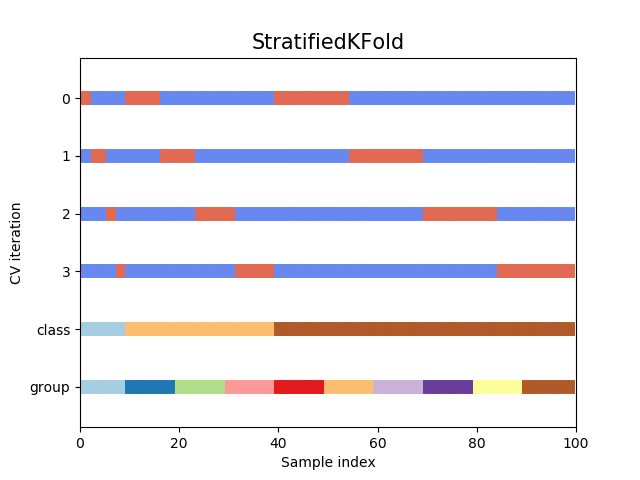
\includegraphics{./fig/strat_kfold.png}
			}
		}
	\end{column}%
\end{columns}
\end{frame}

\begin{frame}{Decritor LBP - Acurácia -10-fold}
\begin{center}
	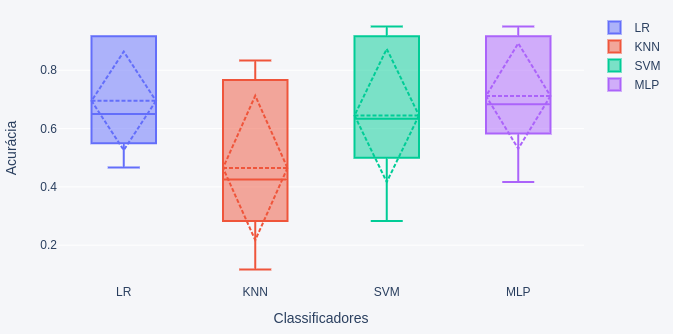
\includegraphics[width=.8\textwidth,height=.7\textheight]{./fig/box_result_lbp.png}
\end{center}
Fonte: \emph{\textcolor{blue}{\href{https://colab.research.google.com/drive/15Ozutw22u9wfAXisgqfhmA33P3s0fbWp?usp=sharing}{Colab}}}
e
\emph{\textcolor{blue}{\href{https://github.com/guimpo/hand_on_again_ai_master/}{GitHub}}}
\end{frame}

\begin{frame}{Decritor Gabor - Acurácia - 10-fold}
\begin{center}
	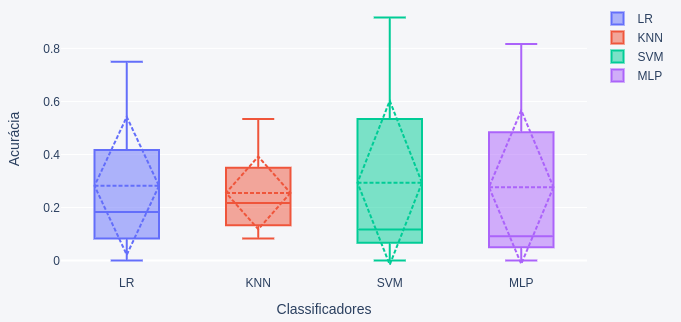
\includegraphics[width=.8\textwidth,height=.7\textheight]{./fig/box_result_gabor.png}
\end{center}
Fonte: \emph{\textcolor{blue}{\href{https://colab.research.google.com/drive/1U0qTE3tIe4U-ODfb8-bq7YlJft0raeHX?usp=sharing}{Colab}}}
e
\emph{\textcolor{blue}{\href{https://github.com/guimpo/hand_on_again_ai_master/}{GitHub}}}
\end{frame}

\begin{frame}{Acurácia - LBP vs Gabor - 10-fold}
\begin{center}
	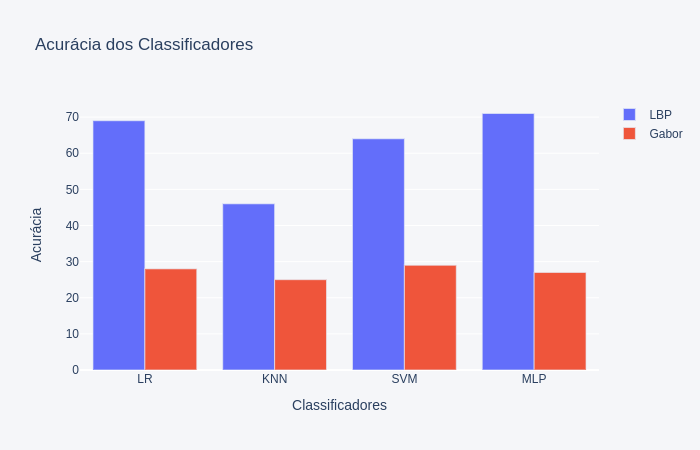
\includegraphics[width=.8\textwidth,height=.7\textheight]{./fig/bar_mean_acc_lbp_vs_gabor.png}
\end{center}
\end{frame}


\begin{frame}{Para onde ir?}
\makebox[\linewidth][c]{
	\resizebox{.6\linewidth}{!}{
		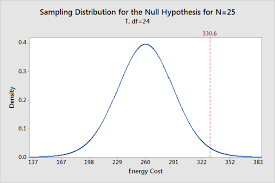
\includegraphics{fig/teste_significancia.png}
	}
}

\hfill%
\begin{wideitemize}
	\item Teste de hipóteses
\end{wideitemize}
\end{frame}